\documentclass{article}

\usepackage{fancyhdr}
\usepackage{extramarks}
\usepackage{amsmath}
\usepackage{amsthm}
\usepackage{amsfonts}
\usepackage{tikz}
\usepackage[plain]{algorithm}
\usepackage{algpseudocode}

\usetikzlibrary{automata,positioning}

\usepackage{graphicx}
\graphicspath{ {./images/} }

%
% Basic Document Settings
%

\topmargin=-0.45in
\evensidemargin=0in
\oddsidemargin=0in
\textwidth=6.5in
\textheight=9.0in
\headsep=0.25in

\linespread{1.1}

\pagestyle{fancy}
\lhead{Yousef Alaa Awad}
\chead{\hmwkClass\: \hmwkTitle}
\rhead{\firstxmark}
\lfoot{\lastxmark}
\cfoot{\thepage}

\renewcommand\headrulewidth{0.4pt}
\renewcommand\footrulewidth{0.4pt}

\setlength\parindent{0pt}

%
% Create Problem Sections
%

\setcounter{secnumdepth}{0}
\newcounter{partCounter}
\newcounter{homeworkProblemCounter}
\setcounter{homeworkProblemCounter}{1}

\newcommand{\hmwkTitle}{Homework\ \#6}
\newcommand{\hmwkClass}{Power Systems Economics}

%
% Title Page
%

\title{
    \vspace{2in}
    \textmd{\textbf{\hmwkClass:\ \hmwkTitle}}\\
    \normalsize\vspace{0.1in}
    \vspace{3in}
}

\author{Yousef Alaa Awad}

% Problems start here
\begin{document}

\maketitle
\pagebreak

\section{4.6}
\textbf{Given:} Borduria GEneration owns three generating units that have the following cost functions:
\begin{itemize}
	\item Unit A: $15+1.4P_A+0.04*P^2_A$ ($\frac{\$}{H}$) 
	\item Unit B: $25+1.6P_B+0.05*P^2_B$ ($\frac{\$}{H}$) 
	\item Unit C: $20+1.8P_C+0.02*P^2_C$ ($\frac{\$}{H}$) 
\end{itemize}
How should these units be dispatched if Borduria Generation must supply a load of 350W at minimum cost?

\subsection{Answer}
With minimum costs, the marginal costs of all units must be equal to a simple system marginal cost, $\lambda$. Therefore we have the following:
$$ MC_A = \frac{dC_A}{dP_A} = 1.4 + 0.08*P_A $$
$$ MC_B = \frac{dC_B}{dP_B} = 1.6 + 0.10*P_B $$
$$ MC_C = \frac{dC_C}{dP_C} = 1.8 + 0.04*P_C $$
After this we simply set $MC_A = MC_B = MC_C = \lambda$, and therefore can rearrange each output in terms of the simple marginal cost ($\lambda$).
$$ P_A = \frac{\lambda - 1.4}{0.08} $$
$$ P_B = \frac{\lambda - 1.6}{0.10} $$
$$ P_C = \frac{\lambda - 1.8}{0.04} $$
After this, we can find the total generation that is the same as the load required (350MW):
$$ \frac{\lambda - 1.4}{0.08} + \frac{\lambda - 1.6}{0.10} + \frac{\lambda - 1.8}{0.04} = 350 \rightarrow $$
$$ 12.5*(\lambda - 1.4) + 10*(\lambda - 1.6) + 25*(\lambda - 1.8) = 350 \rightarrow $$
$$ 47.5*\lambda - 17.5 - 16 - 45 = 350 \rightarrow $$
$$ \lambda = 9.021 $$
Therefore, we now can get the output for each generation unit:
\begin{itemize}
	\item $P_A = \frac{9.021 - 1.4}{0.08} = \textbf{95.3 MW}$
	\item $P_B = \frac{9.021 - 1.6}{0.10} = \textbf{74.2 MW}$
	\item $P_C = \frac{9.021 - 1.8}{0.04} = \textbf{180.5 MW}$
\end{itemize}
Therefore, now we can easily find the hourly total cost, to be simply: 
$$ C(A) + C(B) + C(C) = \textbf{1927.15}\frac{\textbf{\$}}{\textbf{hr}} $$

\subsection{Python Script Output Verification}
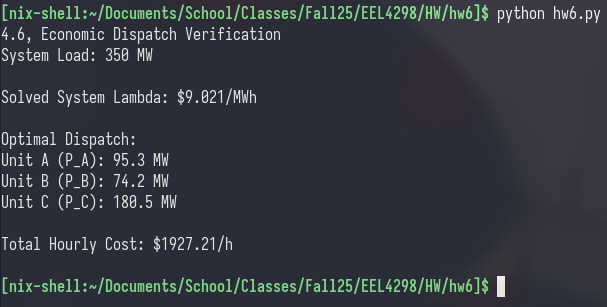
\includegraphics[width=\textwidth]{apple.png}

\section{4.7}
\textbf{Given:} How would the dispatch of Problem 4.6 change if Borduria Generation had the opportunity to buy some of this energy on the spot market at a price of 8.20\$/MWh?
\subsection{Answer}
Now, the dispatch would change due to the fact that Borduria can now buy from the spot market at 8.20$\frac{\$}{MWh}$. This price is, in this case, less than the system's marginal cost calculated in Problem 4.6. This therefore means that it's simply cheaper to buy power rather that generate it at the margin price. This therefore means that the marginal cost of the system is now:
$$ \lambda = 8.20\frac{\$}{MWh} $$
And now, due to this new marginal cost we get a new dispatch of:
\begin{itemize}
	\item $ P_A = \frac{8.20 - 1.4}{0.08} = \textbf{85 MW} $
	\item $ P_B = \frac{8.20 - 1.6}{0.10} = \textbf{66 MW} $
	\item $ P_C = \frac{8.20 - 1.8}{0.04} = \textbf{160 MW} $
\end{itemize}
And now, adding the total generation we get: $85+66+160 = 311\ MW$. Making the remaining load that we have to purchase from the market to be $350 - 311 = \textbf{39 MW}$. This then creates a total cost, when adding the cost of generation and cost of purchase from the market, to be \textbf{1911.20}$\frac{\textbf{\$}}{\textbf{hr}}$.

\section{4.8}
\textbf{Given:} If, in addition to supplying a 350-MW load, Borduria Generation had the opportunity to sell energy on the electricity market at a price of 10.20\$/MWh, what is the optimal amont of power that it should sell? What profit would it derive from this sale?
\subsection{Answer}
Now, when you add the fact that now Borduria has the opportunity to sell energy on the market at a price of 10.20$\frac{\$}{MWh}$, it would mean that its profitable to increase generation and then sell the surplus. This therefore means that the marginal cost will now be set to the market selling price (so that it breaks even in a perfect market):
$$ \lambda = 10.20\frac{\$}{MWh} $$
Therefore the new dispatch is now:
\begin{itemize}
	\item $ P_A = \frac{10.20 - 1.4}{0.08} = \textbf{110 MW} $
	\item $ P_B = \frac{10.20 - 1.6}{0.10} = \textbf{86 MW} $
	\item $ P_C = \frac{10.20 - 1.8}{0.04} = \textbf{210 MW} $
\end{itemize}
This then leads to a total generation of $110+86+210 = 406\ MW$. And the excess amount generated is then sold to the market. That excess being:
$$ 406 - 350 = \textbf{56 MW} $$
This therefore means that, via selling the 56 MW, via producing those required MW makes it so that the company has a \textbf{profit of \$33.03}.

\section{4.9}
\textbf{Given:} Repeat Problem 4.8 if the outputs of the generating units are limited as follows:
\begin{itemize}
	\item $P_A^{MAX} = 100\ MW$
	\item $P_B^{MAX} = 80\ MW$
	\item $P_C^{MAX} = 250\ MW$
\end{itemize}
\subsection{Answer}
Now, since this is a repeat of Problem 4.8, but with differing power generation limits, and that those limits restrict the dispatch that was found in Problem 4.8, the following dispatch will be used:
$$ P_A = \textbf{100 MW}\ (at\ limit) $$
$$ P_B = \textbf{80 MW}\ (at\ limit) $$
$$ P_C = \textbf{210 MW} $$
Now, the total generation is 390 MW. Meaning that the amount sold to the market is...
$$ 390 - 350 = \textbf{40 MW} $$
And, with this sale of 40 MW, and its therefore cost and revenue generated, it would generate a \textbf{profit of \$27.23}.

\end{document}
